\documentclass[12pt]{article}
%\usepackage[utf8]{inputenc}
%\documentclass[UTF8]{ctexart}
%\usepackage[UTF8, heading = false, scheme = plain]{ctex}
\usepackage{geometry}
%geometry{a4paper,scale=0.9}
\geometry{a4paper,left=1cm,right=1cm,top=1cm,bottom=2cm}
\usepackage{amsfonts}
\usepackage{color}
\usepackage{url}
%\usepackage{biblatex}
\usepackage{amsmath}
\usepackage{amssymb}
\usepackage{latexsym}
\usepackage{cite}
%\addbibresource{ref.bib}
%\bibliography{ref.bib}
\usepackage{caption}
\usepackage{graphicx, subfig}
\usepackage{float}
%\usepackage[fontset=ubuntu]{ctex}
%\usepackage{fontspec}
\usepackage{xeCJK}
%\usepackage[colorlinks,
%anchorcolor=black,
%citecolor=black]{hyperref}
%\setmainfont{SimSun}
\usepackage[section]{placeins}
\usepackage{enumitem}
\usepackage{framed}
\usepackage[framemethod=TikZ]{mdframed}
\usepackage{indentfirst}
\usepackage{setspace}%使用间距宏包
\linespread{1.5}
%\title{预备知识}
%\author{leolinuxer }
%\date{June 2020}

\title{使用泰勒公式进行估算时,在不同点有啥区别?\cite{Taylor_Expansion_By_Different_Value}}
\author{leolinuxer}
%\date{June 2020}

\begin{document}
\maketitle

\section{一个问题}
利用函数 $f(x) = x^{\frac{1}{3}}$ 的泰勒展开,可以估算 $30^\frac{1}{3}$ 的值,那么,在 $x = 9$ 处进行展开,和在 $x=27$ 处展开,有什么区别?

\section{泰勒级数的收敛}
\subsection{什么是收敛?}
泰勒公式可以把可导的函数展开为幂级数:
$$
f(x) = f(a) + \frac{f'(a)}{1!} + \frac{f'(a)}{2!}(x-a)^2 + \cdots + \frac{f^(n)(a)}{n!}(x-a)^n + \cdots 
$$

我们对 $f(x) = x^{\frac{1}{3}}$ 进行泰勒展开:
\begin{figure}[H]
  \centering
  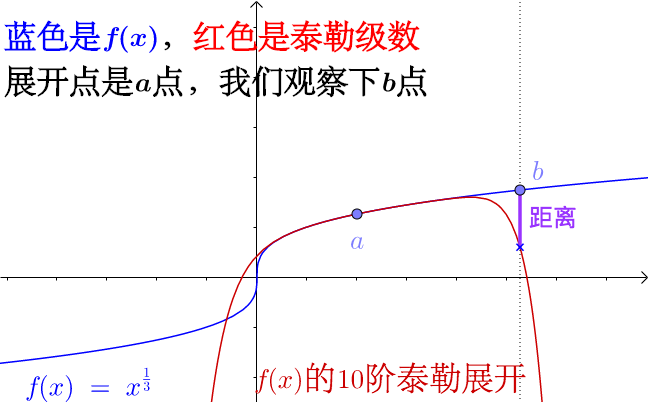
\includegraphics[width=.8\textwidth]{fig/TaylorExpansion_1.png} 
\end{figure}
\begin{figure}[H]
  \centering
  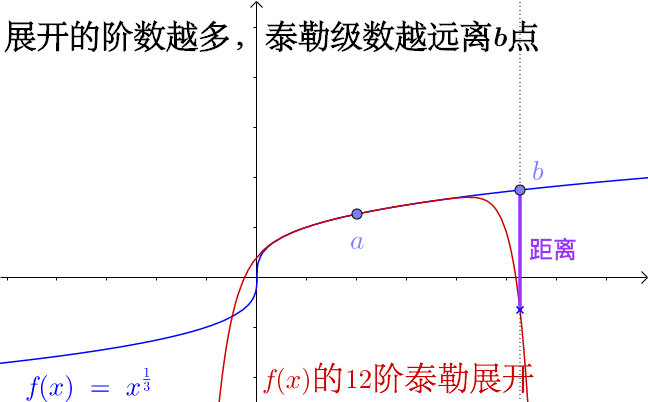
\includegraphics[width=.8\textwidth]{fig/TaylorExpansion_2.png} 
\end{figure}
\begin{figure}[H]
  \centering
  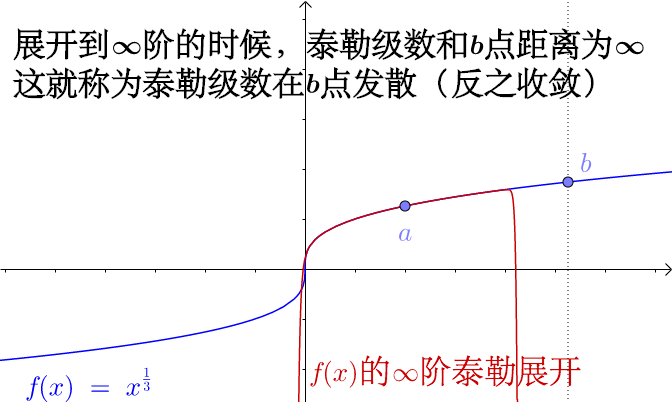
\includegraphics[width=.8\textwidth]{fig/TaylorExpansion_3.png} 
\end{figure}

\subsection{泰勒公式的奇点}
什么叫做奇点?比如对于$f(x)=x^{\frac{1}{3}}$这个函数:
\begin{itemize}
    \item 不可导的点为奇点
    \item 没有定义的点也是奇点
    \item 复平面上的奇点
\end{itemize}
\begin{figure}[H]
  \centering
  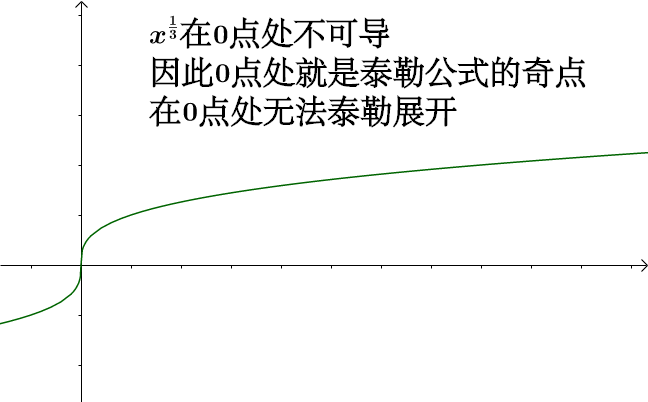
\includegraphics[width=.8\textwidth]{fig/TaylorExpansion_4.png} 
\end{figure}
\begin{figure}[H]
  \centering
  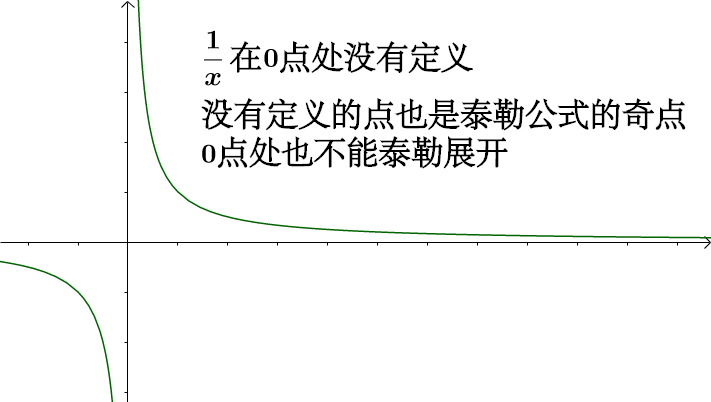
\includegraphics[width=.8\textwidth]{fig/TaylorExpansion_5.png} 
\end{figure}
\begin{figure}[H]
  \centering
  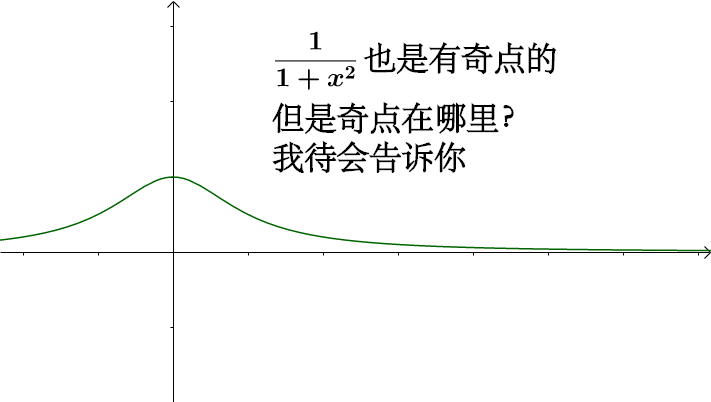
\includegraphics[width=.8\textwidth]{fig/TaylorExpansion_6.png} 
\end{figure}

\subsection{奇点与收敛圆}
通过奇点来判断泰勒级数的收敛,这就是我说的那个非常漂亮的数学结论,由柯西证明的泰勒级数的收敛半径:
\begin{figure}[H]
  \centering
  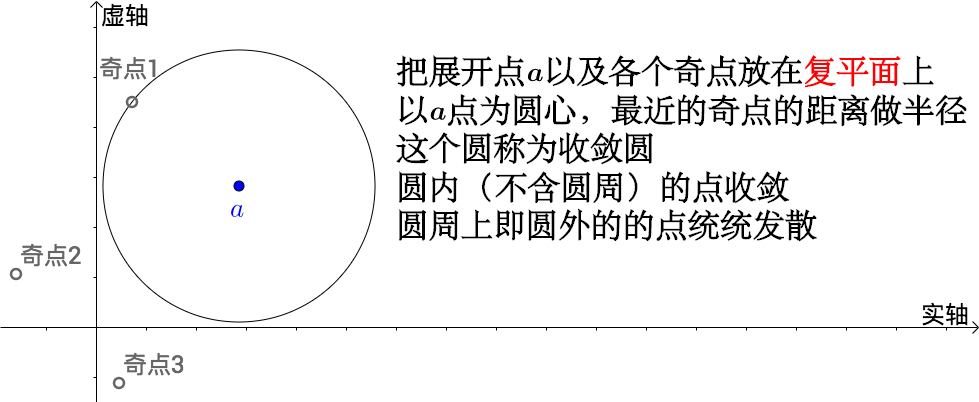
\includegraphics[width=.8\textwidth]{fig/TaylorExpansion_cauchy.png} 
\end{figure}

\textcolor{red}{把展开点 $a$ 以及各个奇点都放在复平面上,以 $a$ 为圆心,最近的奇点的距离做半径,这个圆叫做收敛圆;圆内的点(不含圆周)收敛;圆周上和圆外的点统统发散。}

我们用$f(x)=x^{\frac{1}{3}}$这个函数来举例子:
\begin{figure}[H]
  \centering
  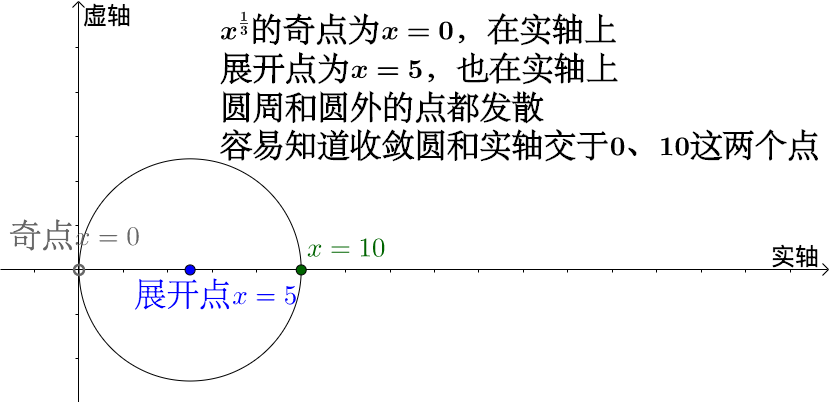
\includegraphics[width=.8\textwidth]{fig/TaylorExpansion_7.png} 
\end{figure}

上面的收敛圆意味着,在实数范围内做$f(x)=x^{\frac{1}{3}}$的话,如果在$x=5处$泰勒展开展开,那么只有在$0 < x < 10$内的泰勒级数才会收敛:
\begin{figure}[H]
  \centering
  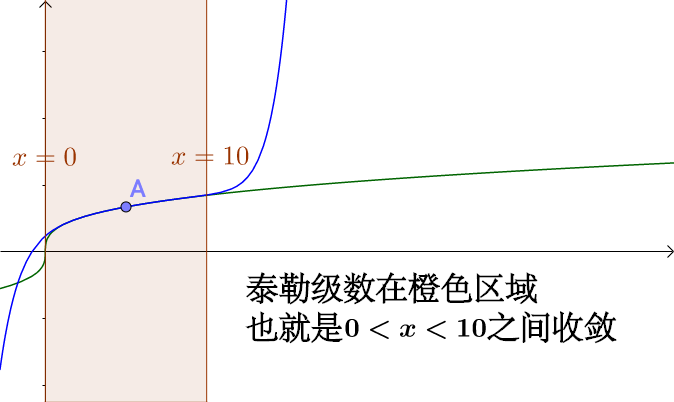
\includegraphics[width=.8\textwidth]{fig/TaylorExpansion_8.png} 
\end{figure}

明白了泰勒公式的收敛半径之后,我们就可以明白:
\begin{figure}[H]
  \centering
  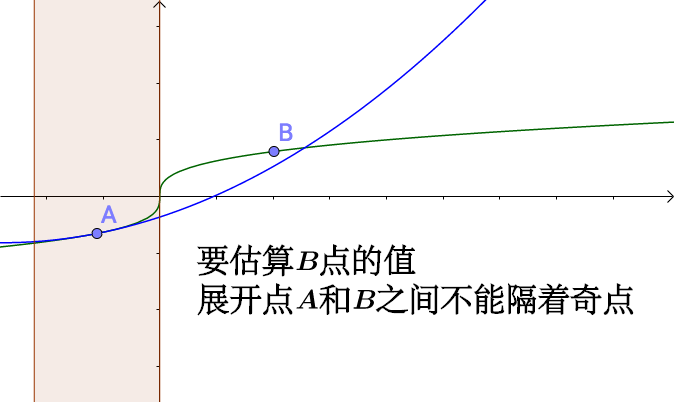
\includegraphics[width=.8\textwidth]{fig/TaylorExpansion_9.png} 
\end{figure}
\begin{figure}[H]
  \centering
  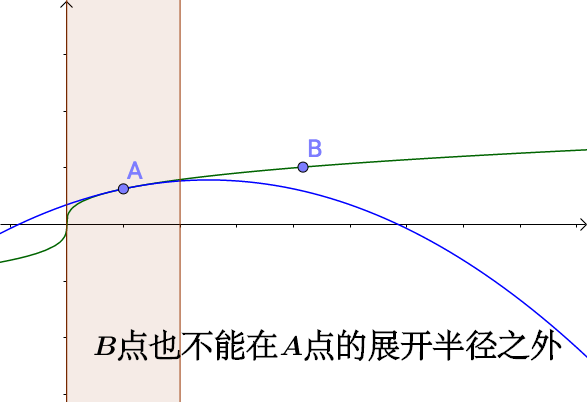
\includegraphics[width=.8\textwidth]{fig/TaylorExpansion_10.png} 
\end{figure}

\subsection{回归到开头的问题}
此时回到我们最初的那个问题:利用函数 $f(x) = x^{\frac{1}{3}}$ 的泰勒展开,可以估算 $30^\frac{1}{3}$ 的值。在 $x = 9$ 处进行展开,$x=30$在收敛半径之外(收敛半径为9),无法估算;在 $x=27$ 处展开,$x=30$在收敛半径之内(收敛半径为27),可以估算。

\subsection{复数与实数的关系}
回到我们之前挖下的坑,$f(x)=\frac{1}{1+x^2}$的奇点在哪里?
很明显$x=i$时,是$f(x)=\frac{1}{1+x^2}$的奇点,因为$1+i^2=0$。我们把奇点和展开点放到复平面上看看:
\begin{figure}[H]
  \centering
  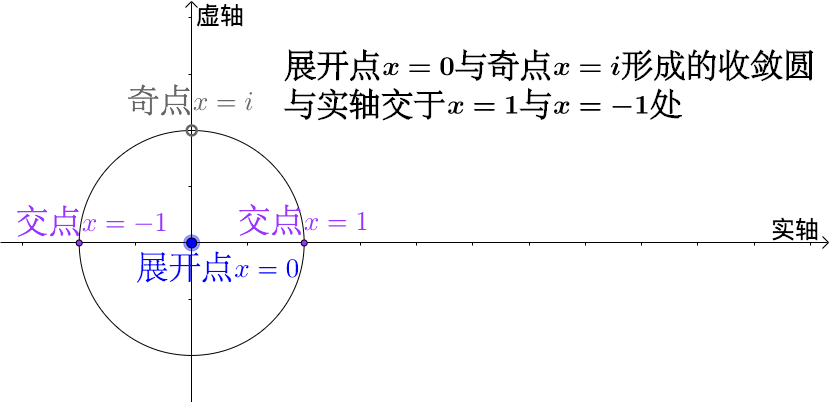
\includegraphics[width=.8\textwidth]{fig/TaylorExpansion_11.png} 
\end{figure}

所以在实平面上的$f(x)=\frac{1}{1+x^2}$,虽然奇点不在实平面内,但是依然被奇点所影响,所以其收敛半径为$-1 < x < 1$:
\begin{figure}[H]
  \centering
  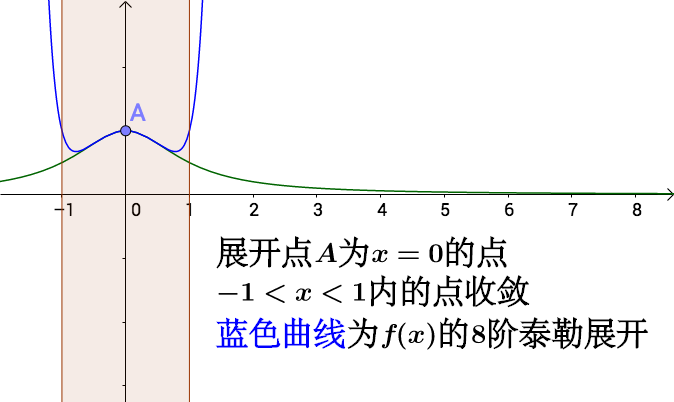
\includegraphics[width=.8\textwidth]{fig/TaylorExpansion_12.png} 
\end{figure}

%\printbibliography
\bibliography{../ref}
\bibliographystyle{IEEEtran}
\end{document}
